\documentclass[a4paper]{article}

%\setlength{\parskip}{0.5\baselineskip}

\usepackage{geometry}
\geometry{left = 2.54 cm, right = 2.54 cm, top = 2.54 cm, bottom = 2.54 cm}

\usepackage{setspace}
\renewcommand{\baselinestretch}{1.0}
\usepackage{indentfirst}
\setlength{\parindent}{2em}

%\usepackage{fontspec}
%\setmainfont{Times New Roman}

\usepackage[]{cprotect}

\usepackage{hyperref}
\hypersetup{
	colorlinks=true,
	linkcolor=blue,
	filecolor=magenta,
	urlcolor=cyan,
}

\usepackage{ulem}
\usepackage{graphicx}
%\usepackage{wrapfig}
\usepackage{enumitem}
\usepackage{xcolor}
\usepackage{subcaption}
\usepackage{float}
\usepackage{amsmath, amssymb, amsthm}
\usepackage{booktabs}

\usepackage{listings} % Required for insertion of code

\lstdefinestyle{lzx}{
		% basicstyle = \small\ttfamily\fontfamily{cmr}\selectfont,
		basicstyle = \ttfamily \footnotesize,
		keywordstyle = \color{purple}\bfseries,
		% commentstyle = \color{green}\itshape,
		commentstyle = \color[RGB]{116, 153, 62}\ttfamily,
		stringstyle = \ttfamily,
		%
		tabsize = 2,
		showspaces = false,
		numberstyle = \ttfamily\color[RGB]{0,96,96},
		showstringspaces = false,
		captionpos = t,
		%
		showlines = true,
		emptylines = *2, % 2 for python, 1 for other language
		numbers = left,
		xleftmargin = 5mm,
		numbersep = 5pt,
		linewidth = \linewidth,
		% backgroundcolor=\color{red},
		frame = single,
		frameround = tttt,
		framexleftmargin = 7mm,
		%
		breaklines = true,
		postbreak = \mbox{\textcolor{red}{\( \hookrightarrow \)}\space},
}

\lstset{
		style = lzx, %
}

%\pagestyle{empty} % Not showing page number

\begin{document}
\renewcommand{\thesection}{\Roman{section}}
\renewcommand{\thesubsection}{\Alph{subsection}}
\renewcommand{\thesubsubsection}{\thesubsection.\arabic{subsubsection}}
\renewcommand{\d}{\: \mathrm{d}}
\newcommand{\e}{\mathrm{e}}

\begin{center}
	\textbf{\Large VE373 Recitation Class}\\[1em]
	\textbf{\large Week 5} \\[1em]
	2022.06.11 \\[1em]
\end{center}

\section{L8 --- Input Capture}
	\par The Input Capture module is useful in applications requiring frequency (period) and pulse measurement.


	\begin{enumerate}[label = \arabic*.]
		\item \textbf{Advantage (comparing to naive solution)}
			\begin{enumerate}[label = \arabic*.]
				\item Accurate
				\item No preemption issue
				\item Don't bother CPU too much
			\end{enumerate}

		\item \textbf{Block diagram}
			\begin{figure}[H]
				\centering
				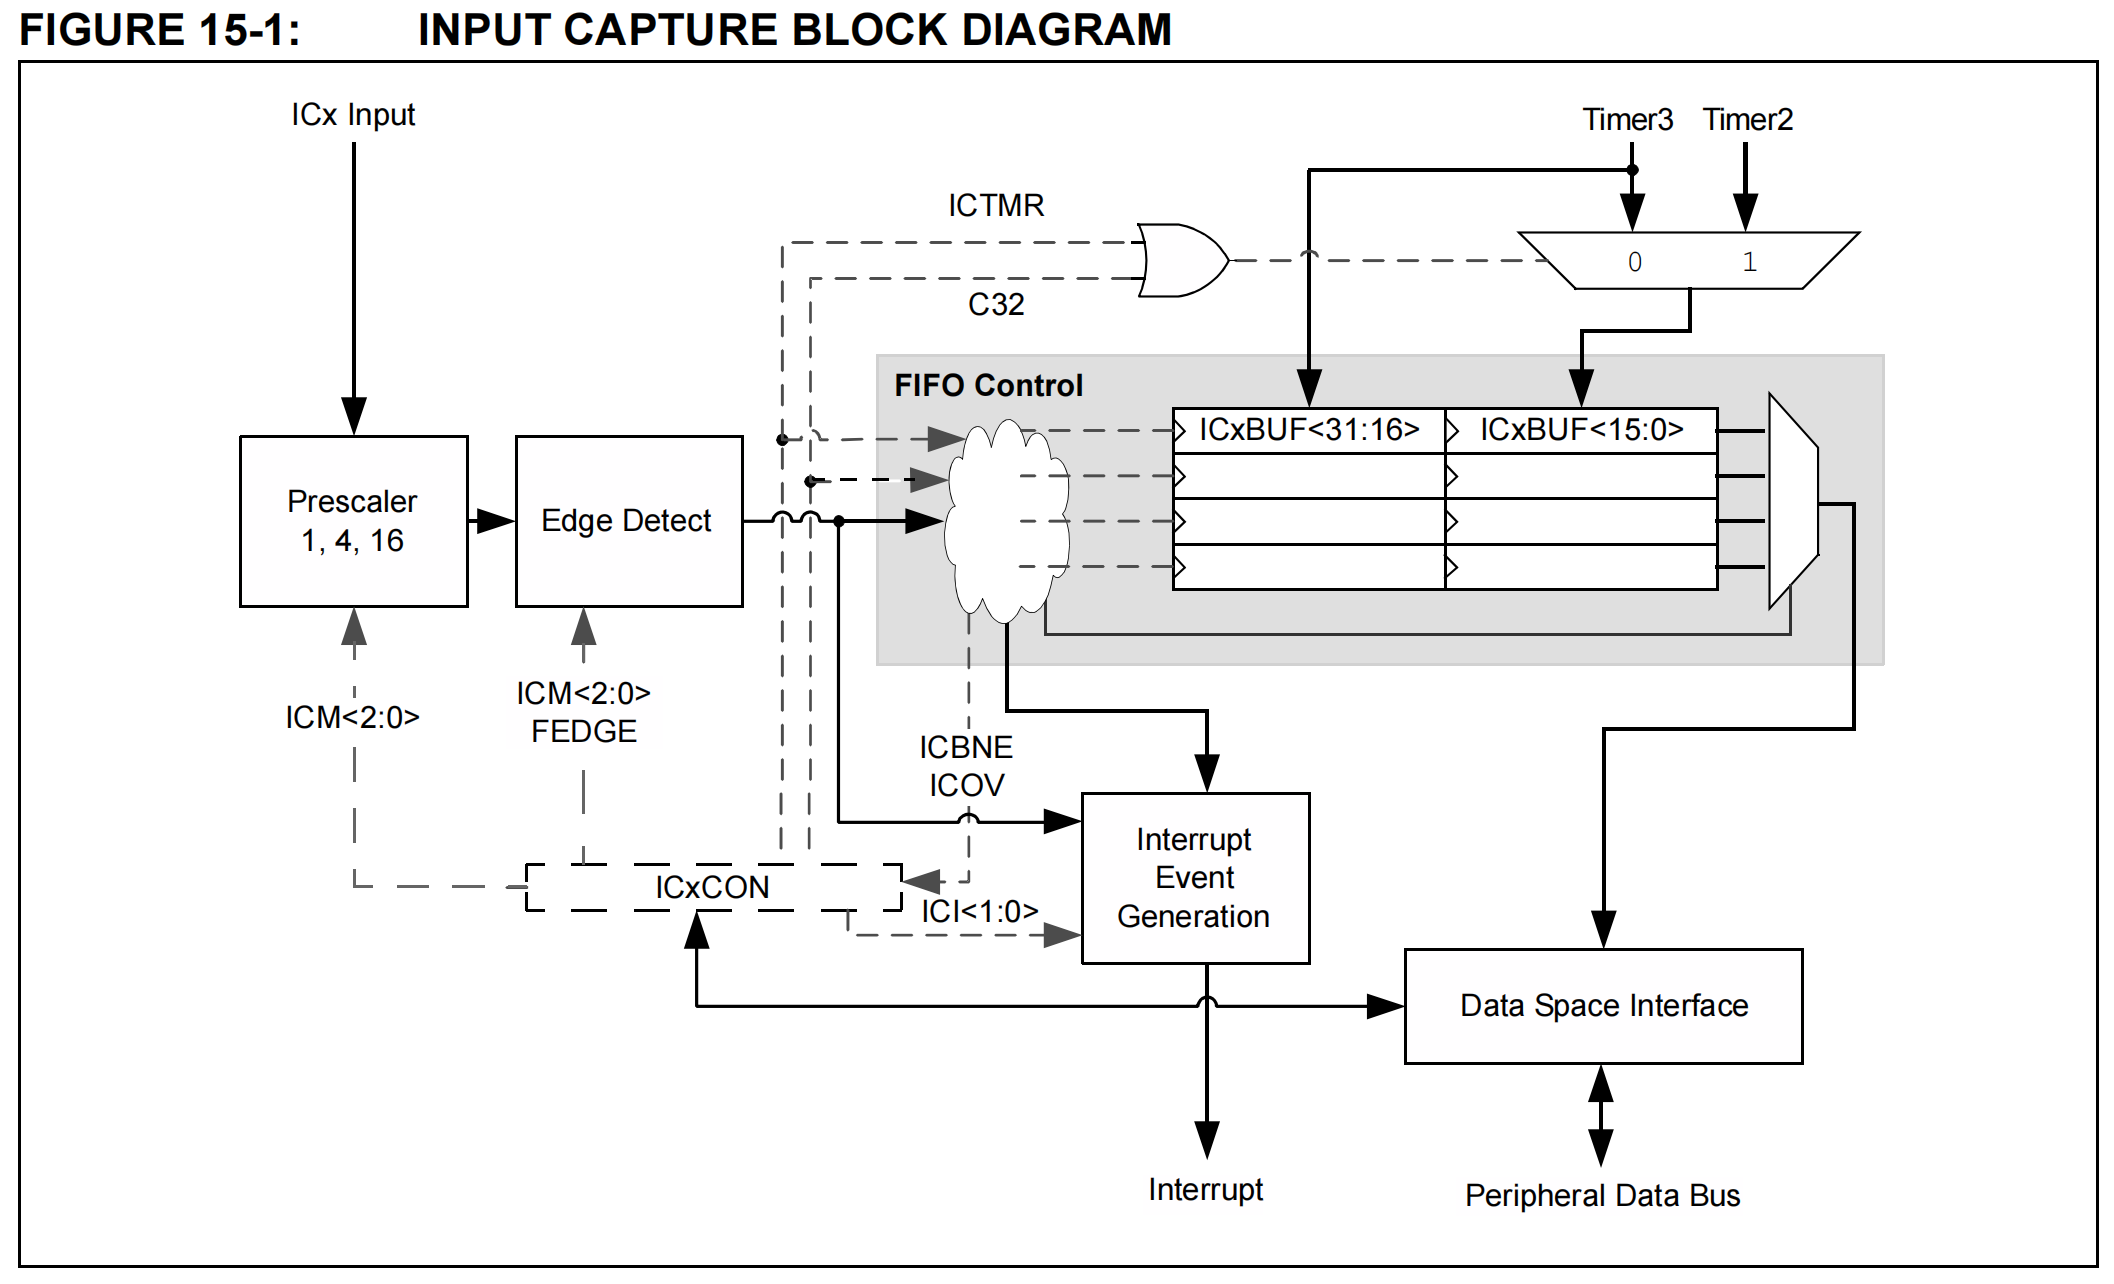
\includegraphics[width=0.9\linewidth]{Input_capture_block_diagram.png}
				\label{fig:Input_capture_block_diagram.png}
			\end{figure}

		\item \textbf{Operation modes}
			\begin{itemize}[leftmargin = 1cm]
				\item Simple capture event modes
					\begin{itemize}[leftmargin = 1cm]
						\item Capture timer value on every falling edge
						\item Capture timer value on every rising edge
						\item Capture timer value on every edge, with specified starting edge (rising or falling)
					\end{itemize}
				\item Prescaled capture event modes
					\begin{itemize}[leftmargin = 1cm]
						\item Capture timer value on every 4th rising edge
						\item Capture timer value on every 16th rising edge
					\end{itemize}
				\item Edge detect mode
				\item Interrupt-only mode
			\end{itemize}

		\item \textbf{Persistent interrupt}
			\par Interrupt is not cleared unless the interrupt condition is cleared.
			\begin{figure}[H]
				\centering
				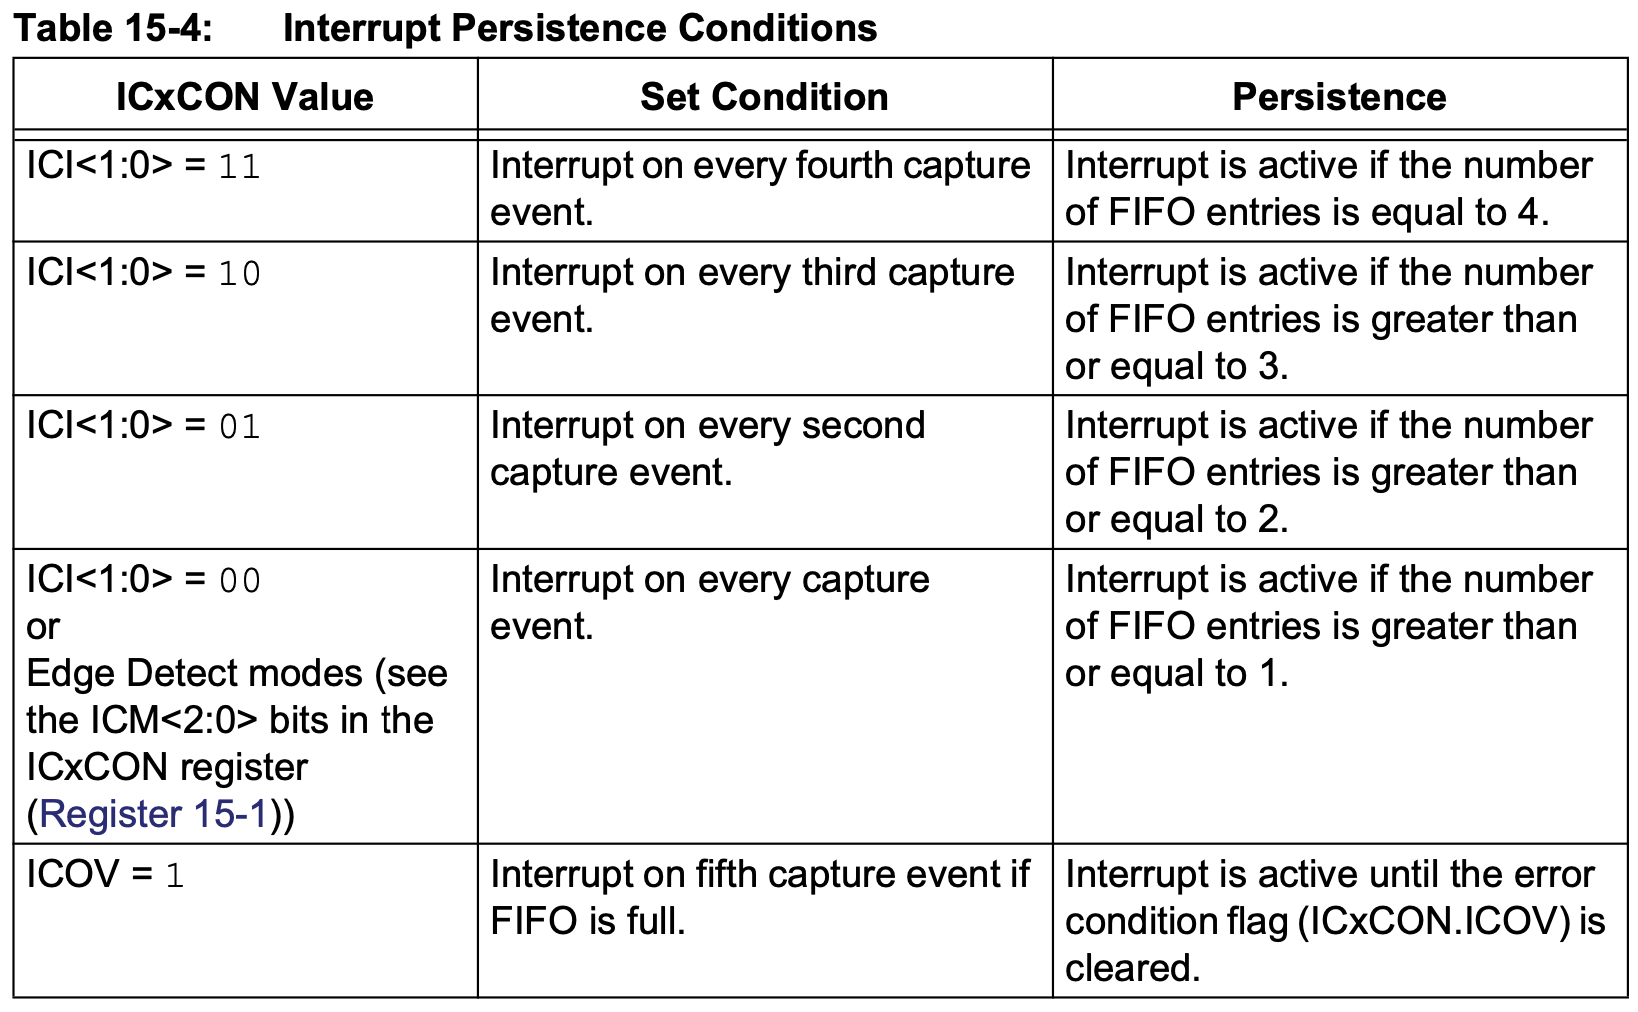
\includegraphics[width=0.6\linewidth]{Input_capture_persistent_condition.png}
				\label{fig:Input_capture_persistent_condition.png}
			\end{figure}

		\item \textbf{Simple capture event modes}
			\begin{itemize}[leftmargin = 1cm]
				\item 2--3 \( T_{PB} \) delay after the event due to synchronization
				\item Capture input is sampled by \verb|PBCLK|, therefore input signal high and low width \( >T_{PB} \).
			\end{itemize}

		\item \textbf{Edge Detect Mode}
			\begin{itemize}[leftmargin = 1cm]
				\item Prescaler and interrupt count not used.
				\item Buffer overflow never signals.
				\item Interrupt request on every capture.
			\end{itemize}

		\item \textbf{Interrupt-only mode}
			\begin{itemize}[leftmargin = 1cm]
				\item Rising edge on ICx triggers an interrupt
					\begin{itemize}[leftmargin = 1cm]
						\item Not functioning during normal operation
						\item No timer capture
						\item No buffer update
					\end{itemize}
				\item Used only as a wake-up mechanism for SLEEP or IDLE modes
			\end{itemize}

		\item \textbf{Capture buffer flags}
			\begin{itemize}[leftmargin = 1cm]
				\item \verb|ICBNE| (\verb|ICxCON<3>|): IC buffer not empty
					\begin{itemize}[leftmargin = 1cm]
						\item Read-only
						\item Signals when 1 or more entries
					\end{itemize}
				\item \verb|ICOV| (\verb|ICxCON<4>|): IC buffer overflow
					\begin{itemize}[leftmargin = 1cm]
						\item Signals on the 5th capture
						\item All extra capture values are lost, until flag cleared
						\item Flag cleared when
							\begin{itemize}[leftmargin = 1cm]
								\item IC Module disabled
								\item Module reset
								\item \verb|ICBNE| becomes 0 --- IC buffer empty
							\end{itemize}
					\end{itemize}
			\end{itemize}


		\item \textbf{Capture event and interrupt event}
			\begin{itemize}[leftmargin = 1cm]
				\item Capture event: capture change of \verb|ICx| and store timer value in the FIFO\@.
				\item Interrupt event: interrupt after certain amount of capture events.
			\end{itemize}

		\item \textbf{Examples}
			\par See reference manual or slides.
	\end{enumerate}


\section{L9 --- Output Compare and PWM}
	\par The Output Compare module is used to generate a single pulse or a series of pulses in response to selected time base events.
	\begin{enumerate}[label = \arabic*.]
		\item \textbf{Block diagram}
			\begin{figure}[H]
				\centering
				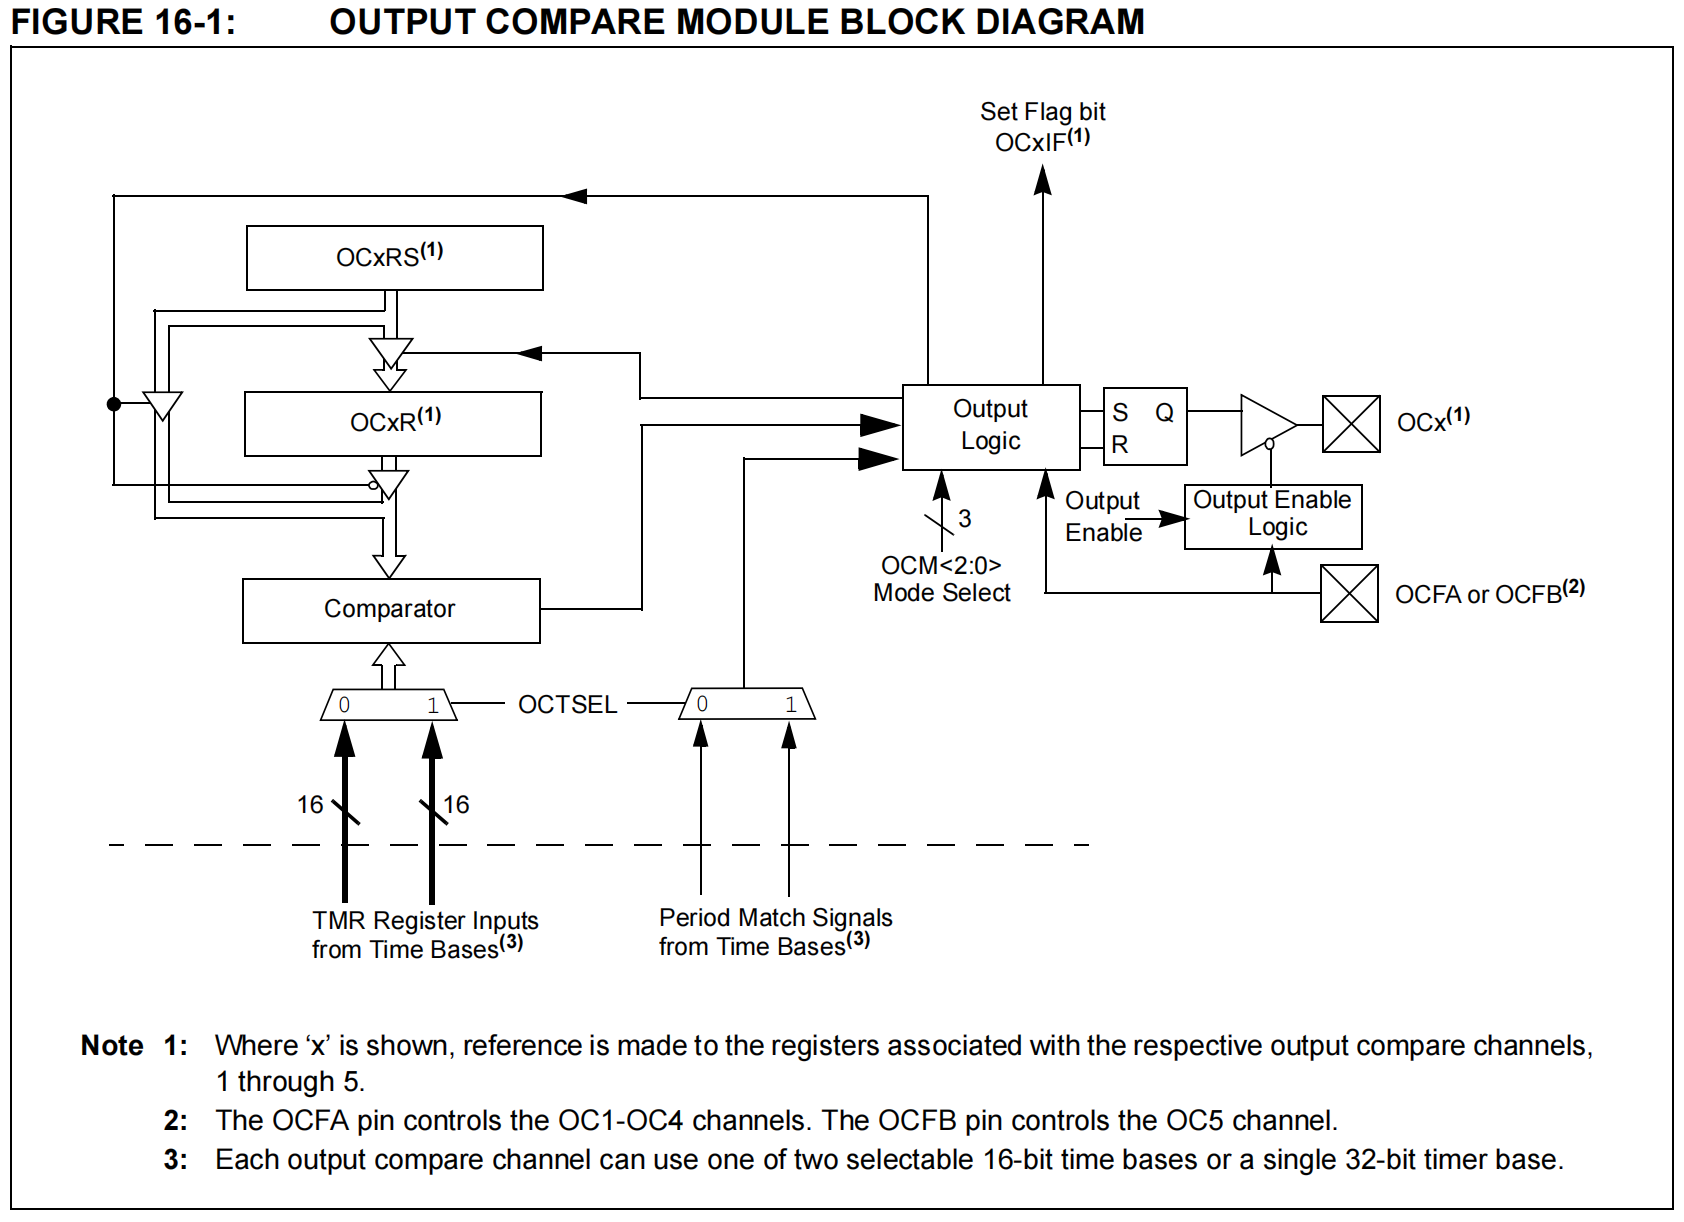
\includegraphics[width=0.9\linewidth]{Output_compare_block_diagram.png}
				\label{fig:Output_compare_block_diagram.png}
			\end{figure}

		\item \textbf{Operation mode}
			\begin{itemize}[leftmargin = 1cm]
				\item Single Compare Match mode
					\par Drive high, drive low, toggle
				\item Dual Compare Match mode
					\par Single output pulse, continuous output pulses
				\item Simple Pulse Width Modulation (PWM) mode
					\par With or without fault protection input
			\end{itemize}

		\item \textbf{Single Compare Match mode}
			\begin{itemize}[leftmargin = 1cm]
				\item Compare forces \verb|OCx| pin high; initial state of pin is low. Interrupt is generated on the single compare match event.
				\item Compare forces \verb|OCx| pin low; initial state of pin is high. Interrupt is generated on the single compare match event.
				\item Compare toggles \verb|OCx| pin. Toggle event is continuous and an interrupt is generated for each toggle event.
			\end{itemize}

		\item \textbf{Dual Compare Match mode}
			\par Single or continues pulse.

		\item \textbf{Single pulse special situations}
			\begin{itemize}[leftmargin = 1cm]
				\item \verb|PRy >= OCxRS > OCxR = TMRy = 0|
					\par The initial match of \verb|OCxR| and \verb|TMRy| at 0 doesn't drive high, work normally afterwards
				\item \verb|PRy >= OCxR >= OCxRS|
					\par Match \verb|OCxR| first, match \verb|OCxRS| in next counting round
				\item \verb|OCxRS > PRy >= OCxR|
					\par Only rising edge generated on first match, then signal remains high, no interrupt generated
				\item \verb|OCxR > PRy|
					\par Not working, \verb|OCx| remains low
			\end{itemize}

		\item \textbf{PWM mode}
			\par Covered in next RC\@.

		\item \textbf{Examples}
			\par See reference manual or slides.
	\end{enumerate}


\end{document}